%%%%%%%%%%%%%%%%%%%%%%%%%%%%%%%%%%%%%%%%%%%%%%%%%%%%%%%%%%%%%%%%%%% 
%                                                                 %
%                           CHAPTER 4                             %
%                                                                 %
%%%%%%%%%%%%%%%%%%%%%%%%%%%%%%%%%%%%%%%%%%%%%%%%%%%%%%%%%%%%%%%%%%% 
 
\chapter{Dramatic inner-core tropopause variability during the rapid intensification of {Hurricane Patricia} (2015)}
\resetfootnote %this command starts footnote numbering with 1 again.

%---------------------------------------------------------------------------------------%
\section{Introduction}
%---------------------------------------------------------------------------------------%

Hurricane Patricia became the strongest recorded hurricane in the Western Hemisphere after undergoing remarkably rapid intensification (RI) between 21 and 23 October 2015 (\citeauthor{Kimberlainetal2016} \citeyear{Kimberlainetal2016}; \citeauthor{Rogersetal2017} \citeyear{Rogersetal2017}).

Throughout this RI period, a NASA WB-57 aircraft flying in the stratosphere deployed 244 dropsondes as part of the Office of Naval Research Tropical Cyclone Intensity (TCI) Experiment \cite{DoyleTCI}.
These dropsondes revealed dramatic changes in upper-level static stability and cold-point tropopause structure throughout Patricia’s RI.

%---------------------------------------------------------------------------------------%
\section{Data and methods}
%---------------------------------------------------------------------------------------%
The High-Definition Sounding System (HDSS) provides a new capability to deploy and track up to 40 expendable digital dropsondes (XDDs) simultaneously.
This capability permits the rapid deployment of many dropsondes, providing cross sections of pressure, temperature, humidity, and wind velocity with unprecedented horizontal resolution.
\cite{Blacketal2017} report that XDDs are able to resolve atmospheric features in a manner comparable to RD-94 dropsondes \cite{HockFranklin1999}, operational rawinsondes, and aircraft spiral profiles.
The XDDs exhibited a warm bias of 18C and a dry bias of 5\% relative to RD-94 dropsondes.
XDD thermodynamic measurements, like those of other in situ sounding instruments, were noisy and unreliable when the sensors became wet.
An intensive quality control procedure \cite{BellTCI} removed unrealistic temperature and humidity observations that likely reflected sensor wetting, as well as relative humidity recorded at temperatures below -40\textdegree{}C, where humidity measurements were inaccurate because of slow sensor response time.
A more complete description of HDSS’s specifications and error characteristics can be found in \cite{Blacketal2017} and \cite{DoyleTCI}, and a comprehensive description of tihe quality control procedure in \cite{BellTCI}.

Flying near 18.5-km altitude aboard the NASA WB-57 aircraft, HDSS deployed dropsondes with horizontal spacing as small as 4 km in the inner core of TC Patricia.
This dataset builds upon that of the high-altitude dropsonde observations collected by the NASA Hurricane and Severe Storm Sentinel (HS3) investigation \cite{Braunetal2016}.
Although many dropsondes were deployed during each HS3 flight, the typical spacing of 50–200 km was not sufficient to resolve the inner core of a hurricane. In contrast, the average dropsonde spacing for the four complete transects that TCI conducted through the center of TC Patricia ranged from 4.4 to 8.0 km. 
These four flight legs, shown in Fig.~\ref{fig:patricia_ir}, will be used to analyze the upper-tropospheric and lower-stratospheric evolution of TC Patricia during its RI.

The infrared (IR) brightness temperature images plotted in Fig.~\ref{fig:patricia_ir} were parallax-corrected using Man
computer Interactive Data Access System (McIDAS-X; \citeauthor{Lazzaraetal1999} \citeyear{Lazzaraetal1999}), assuming a cloud-top height of 15 km.
For each transect, the parallax adjustment was determined at every dropsonde position and the IR image was shifted by the average of these adjustment factors.
This effectively shifted the IR image 9 km to the southeast on 21 October (when the satellite image came from GOES-13) and 13 km to the southwest on 22 and 23 October (when the satellite image came from GOES-15).
This parallax adjustment was performed only to show more realistic dropsonde deployment locations relative to the IR brightness temperatures in Fig.~\ref{fig:patricia_ir}; it did not impact any calculated field.

Each sounding in the quality-controlled TCI dropsonde dataset \citep{BellTCI} was interpolated to a 100-m vertical grid following \cite{MolinariVollaro2010}.
The static stability was analyzed using the squared Brunt–V{\"a}is{\"a}l{\"a} frequency:
   \begin{equation} \label{eq:n2dry}
   N^2 = \frac{g}{\theta}\frac{\Delta \theta}{\Delta z},
   \end{equation}
where $\Delta z$ is 200 m.
The vertical temperature gradient, $\Delta T/\Delta z$, also was computed across 200-m layers using centered finite differences.

The evolution of $\theta$ anomalies will be used to aid the diagnosis of static stability changes.
Although many previous papers have used the \cite{Jordan1958} or \cite{Dunion2011} mean soundings to compute temperature anomalies, neither of these soundings are representative of the environment in which Patricia was embedded.
For this reason, a mean state was defined using an average of 74 rawinsonde observations obtained from the University of Wyoming upper-air sounding archive \citep{Wyoming2016}.
These observations constituted all rawinsondes released from Manzanillo and Acapulco, Mexico, during October 2015. Each sounding was visually inspected for errors and three soundings from Manzanillo were removed from the average: 0000 UTC 6 October, 1200 UTC 11 October, and 1200 UTC 21 October.
These soundings exhibited unrealistically large upper-tropospheric temperature departures relative to the previous and subsequent soundings.
Their removal did not significantly alter the mean sounding: the maximum difference in the average temperatures computed with and without those soundings was 0.47\textdegree{}C. 
A total of 58 of the 74 rawinsondes reported data up to at least the 19-km level, facilitating the computation of $\theta$ anomalies well into the lower stratosphere.

For each cross section, the storm center location was determined using a wind center track produced by NOAA’s Hurricane Research Division (available online at \url{http://www.aoml.noaa.gov/hrd/Storm_pages/patricia2015/patricia.trak}).
The WB-57 dropsonde deployment location nearest this storm center estimate in space and time was used to define the center (radius = 0) for each cross section.
The distance between the nearest dropsonde and the storm track never exceeded 8.1 km (Table~\ref{table1}).
Storm-relative radial and tangential velocities were computed using the speed and direction of motion along this track.

%---------------------------------------------------------------------------------------%
\section{Results}
%---------------------------------------------------------------------------------------%

The center-crossing transects on 21, 22, and 23 October 2015 are shown in Figs. \ref{fig:patricia_ir}a-d, overlaid on infrared brightness temperature images from GOES.
Stars indicate dropsonde deployment locations and range rings are plotted every 20 km.
Brightness temperatures colder than -80\textdegree{}C extended over a broad region of Patricia’s circulation on 21 October (Fig. \ref{fig:patricia_ir}a, pink shading).
Convection was asymmetric about the storm center, with the coldest brightness temperatures (colder than -86\textdegree{}C) confined to a region 60–80 km west of Patricia’s center of circulation.
By 22 October, Patricia had rapidly intensified to a category 3 hurricane (Fig. \ref{fig:vmax}), with an eye beginning to clear in the infrared (Figs. \ref{patricia_ir}b,c).
This rapid intensification continued over the next 18 h until the storm’s maximum sustained wind speed reached its peak
of 185 kt (1 kt = 0.5144 m s\textsuperscript{-1}) at 1200 UTC 23 October (Fig. \ref{fig:vmax}; \citeauthor{Kimberlainetal2016} \citeyear{Kimberlainetal2016}).
TCI conducted its final flight into Patricia shortly thereafter, crossing over the eye around 2000 UTC (Fig. \ref{fig:patricia_ir}d) as the storm begain to weaken.

The tropopause temperature, pressure, and $\theta$ observed along these four transects (Fig. \ref{fig:trop}) exhibit strong spatial and temporal variability.
On 21 October, the tropopause temperature (Fig. \ref{fig:trop}a, blue line) was colder than -80\textdegree{}C at all radii.
The coldest tropopause temperature observed, -84\textdegree{}C, was located about 45 km west of the storm center, within a region of IR brightness temperatures between -84\textdegree{} and -86\textdegree{}C.
These cold tropopause temperatures west of the storm center tended to be associated with lower tropopause pressure (Fig. \ref{fig:trop}b, blue line).
On this day, tropopause $\theta$ (Fig. \ref{fig:trop}c, blue line) varied from 374 K east of the storm center to 385 K west of the storm center.
By 22 October (green and orange lines), all three tropopause quantities had changed dramatically.
The tropopause temperature increased everywhere, and at the storm center temperature rose from near -83\textdegree{}C on 21 October to -77\textdegree{}C in the first transect on 22 October (Fig. \ref{fig:trop}a, green line).
During this same period, the tropopause pressure at the storm center decreased from 93 to 85 hPa.
This combination of increasing temperature and decreasing pressure led to a $\theta$ increase of greater than 20 K at the tropopause.
The dropsonde deployed nearest Patricia’s center of circulation during the second transect (orange lines) was missing all data above 11.7 km.
However, another dropsonde deployed on the northeast edge of the eye observed a tropopause pressure and temperature of 79 hPa and -77\textdegree{}C, respectively.
This corresponded to a tropopause $\theta$ of 406 K, which was 31 K higher than that observed at the storm center less than 24 h prior.
These trends continued into 23 October (red lines), by which time the tropopause temperature at the storm center had increased to -72\textdegree{}C and the pressure approached 75 hPa---the highest available data point---in two dropsondes deployed near the southeast edge of the eyewall.

Cross sections of $\Delta T/\Delta z$ [K (100 m)\textsuperscript{-1}; Figs. \ref{fig:stab}a–d] and $N^2$ (10\textsuperscript{-4} s\textsuperscript{-2}; Figs. \ref{fig:stab}e–h) reveal dramatic changes in the static stability structure near the tropopause during Patricia’s RI.
On 21 October (Fig. \ref{fig:stab}a), the cold-point tropopause was located between 16.9 and 17.4 km---a few hundred meters higher than the annual-mean tropopause height in the tropical east Pacific (see \citeauthor{Seideletal2001} \citeyear{Seideletal2001}, their Fig. 4a).
A strong TIL (inversions represented by red shading) existed immediately above the tropopause, with temperature increasing upward by 2 K (100 m)\textsuperscript{-1} over a broad region of the circulation.
This inversion was similar in magnitude to those observed by \cite{Gentry1967} and \cite{Waco1970} in Hurricanes Isbell (1964) and Beulah (1967), and manifested as a 500-m-thick ribbon of N2 greater than 10\textsuperscript{-3} s\textsuperscript{-2} (Fig. 4e).
The inversion was strongest in the vicinity of the coldest cloud tops (Fig. \ref{fig:patricia_ir}a), reaching magnitudes greater than 4.5 K (100 m)\textsuperscript{-1} at four locations west of the storm center.
Three of these maxima were accompanied by 100-m upward spikes in tropopause height and stronger lapse rates just below the tropopause than were observed outside of the coldest cloud tops.
The dropsondes with the strongest inversions---dropsondes 13 and 15---were deployed within the region of coldest IR brightness temperature 40–80 km west of the center.
This suggests some connection between the presence of localized deep convection and a strong TIL, which will be discussed in section \ref{sec:discussion}.

By 1823 UTC 22 October (Fig. \ref{fig:stab}b), the TIL had thinned and weakened considerably, particularly near the storm center.
Between 10- and 20-km radius on each side, near the outer edge of the eye, the temperature profile became approximately isothermal above about 16.6 km.
These isothermal layers corresponded to slightly larger static stability in the 16.5–17-km layer than was observed on the previous day, but smaller static stability above 17 km (cf. Figs. \ref{fig:stab}e,f).
The decay of the TIL during this period allowed the tropopause height to increase at and southeast of the storm center, as can be seen by comparing the blue and green lines in Fig. \ref{fig:trop}b.
Northwest of the storm center, meanwhile, the static stability below 17 km increased, and the tropopause height decreased. Some remnants of the TIL remained, with a small region marked by a 2 K (100 m)\textsuperscript{-1} temperature inversion 70–80 km northwest of the storm center.
Localized areas of large static stability also were present in the 17.5–18.5-km layer.

Forty minutes later, a southwest–northeast transect observed a similar structure in the southwestern quadrant of the storm, with a temperature inversion persisting outside of the 40-km radius (Fig. \ref{fig:stab}c).
In the eye region, however, the TIL had eroded further and the tropopause height increased to 18 and 18.1 km southwest and northeast of the center, respectively.
Although the dropsonde deployed nearest the storm center and the dropsonde deployed just to its southwest are missing data in the tropopause layer, two dropsondes near the edge of the eye---dropsondes number 14 and 17---observed a nearly isothermal layer extending from 16.7 km upward to 18 km.
The transition from an inversion layer on 21 October to an isothermal layer on 22 October was associated with decreasing static stability in the eye region during this period (cf. Figs. \ref{fig:stab}e,g) and an increase in tropopause height.
Southwest of the eye, a persistent TIL limited the tropopause height to the layer between 17 and 17.5 km, and northeast of the eye, between 16.7 and 16.9 km (Fig. \ref{fig:stab}c).
The asymmetry in tropopause height is coincident with a convective asymmetry characterized by coldest brightness temperatures southwest of the storm center and warmest brightness temperatures northeast of the storm center (Fig. \ref{fig:patricia_ir}c).

On 23 October (Figs. \ref{fig:stab}d,h), the tropopause reached 18.3 km---the maximum level of available data---in two soundings through Patricia’s eye (dropsondes 33 and
34).
This represents a further increase in tropopause height over the eye between 22 and 23 October, and was associated with decreasing static stability during that period within the 20-km radius (cf. Figs. \ref{fig:trop}g,h).
In contrast, no sounding outside of the 20-km radius observed a tropopause higher than 17.5 km.
These regions saw a restrengthening of the TIL, with a large number of dropsondes once again observing temperature inversions of magnitude greater than 2 K (100 m)\textsuperscript{-1}, especially above the eyewall regions near 70 km northwest and 30 km southeast of the storm center.
These regions also were marked by local maxima in tropopause height.
Near 10--20-km radii on each side of the storm center, like the previous day, there was a layer of nearly zero $\Delta T/\Delta z$, extending down to the 16.2-km level, which was deeper into the troposphere than on the previous day.
It is unclear what caused these quasi-isothermal layers on the outer edge of the eye, but their existence complicates the definition of the tropopause.
For example, the cold-point tropopause height in dropsonde number 28 was 16.3 km, where the temperature reached its minimum of -72.12\textdegree{}C.
The same dropsonde, however, observed a temperature of -72.07\textdegree{}C at 17.8 km.
The difference between these two temperatures was well within the margin of error of the dropsonde temperature sensor (0.5\textdegree{}C; \citeauthor{BellTCI} \citeyear{BellTCI}).
Thus, the cold-point tropopause might have been much higher at these locations and we do not attribute any significance to the sharp, localized drops in tropopause height on each side of the eye.
In contrast, the presence of an elevated tropopause over the eye in multiple soundings on 22 and 23 October, together with the systematic increase in tropopause height throughout the observation period, lends confidence that the elevated tropopause over the eye is a real signal.

Cross sections of $\theta$ are shown in Figs. \ref{fig:anomalies}a--d and $\theta$ anomalies in Figs. \ref{fig:anomalies}e–h.
On 21 October, a broad region of Patricia’s inner core exhibited $\theta$ anomalies colder than -4 K at and just below the tropopause (Fig. \ref{fig:anomalies}e).
Immediately above this anomalous cold layer existed a layer with warm anomalies greater than 8 K.
This anomalous warm layer, combined with the anomalous cold layer at and below the tropopause, helped to produce the particularly well-defined TIL observed on 21 October (Fig. \ref{fig:stab}a).
As Patricia’s RI commenced, an upper-tropospheric warm core began to develop within
the 30-km radius.
For example, the maximum $\theta$ at the 16-km level increased from approximately 368 K on 21 October (Fig. \ref{fig:anomalies}a) to 378 K on 22 October (Fig. \ref{fig:anomalies}c).
Meanwhile, the horizontally extended cold anomaly at and just beneath the tropopause weakened considerably, as did the warm anomaly in the lower stratosphere.
Just above the tropopause to the northeast of the storm center, however, a warm anomaly of up to 8 K remained (Fig. \ref{fig:anomalies}g), along with a cold anomaly of up to 4 K immediately surrounding the tropopause.
Later in the RI period (22--23 October), Patricia’s warm core developed more rapidly, with the strongest warming confined to within 20 km of the storm center.
By 23 October, upper-tropospheric $\theta$ within the eye exceeded 400 K---a value previously found only in the lower stratosphere.
Oscillations in $\theta$, possibly inertia--gravity waves, are evident to the northwest of the eye just radially outside of the secondary eyewall (Fig. \ref{fig:anomalies}d), extending from 60 km to at least 130 km northwest of the storm center.
These waves affected the static stability all the way up to 18 km (Fig. \ref{fig:stab}h), caused 100--200-m fluctuations in the tropopause height, and were associated with oscillations in radial and tangential velocity (not shown).
A detailed analysis of these waves is outside of the scope of this paper, but to our knowledge this may be the first time that inertia--gravity waves have been resolved by dropsondes in a hurricane.

Changes in $\theta$ over 24 h (Fig. \ref{fig:dtheta}) highlight two distinct periods of $\theta$ evolution during Patricia’s RI.
Figure \ref{fig:dtheta}a shows the change in $\theta$ between 21 and 22 October (Fig. \ref{fig:anomalies}b minus Fig. \ref{fig:anomalies}a) and Fig. \ref{fig:dtheta}b the $\theta$ change between 22 and 23 October (Fig. \ref{fig:anomalies}d minus Fig. \ref{fig:anomalies}b).\footnote{We have chosen to use only the first transect on 22 October (Fig. \ref{fig:patricia_ir}b) because it sampled the same quadrants as the center-crossing transects on 21 and 23 October; difference fields using the second, southwest--northeast, transect on 22 October (Fig. \ref{fig:patricia_ir}c) are qualitatively similar (not shown).}
The differences are scaled to 24 h by multiplying by $24/\Delta t$, where $\Delta t$
is the time (in hours) separating the center crossings of the two transects.
During the early part of Patricia’s RI (Fig. \ref{fig:dtheta}a), $\theta$ decreased dramatically above the 17.5-km level, with cooling greater than 10 K observed at nearly all radii over a 24-h period.
A radially extensive region of warming existed just a few hundred meters below this strong cooling, with $\theta$ increases of at least 4 K observed at nearly all radii.
These $\theta$ increases maximized in the 17.0--17.4-km layer---the layer in which the tropopause was located throughout much of the cross section (see Figs. \ref{fig:stab}a,b).
Later in the RI period (Fig. \ref{fig:dtheta}b), $\theta$ increased over almost the entire domain, including in the lower stratosphere up to at least 18.4 km.
These increases no longer maximized in a thin, horizontally extended layer near the tropopause; rather, the largest $\theta$ changes were confined to a region within 30 km of the storm center.
Maximum $\theta$ tendencies flanked the storm center on each side, consistent with the ‘‘warm ring’’ noted by \cite{Schubertetal2007} and \cite{SternZhang2013}.
Within the eye region (radius <20 km), the magnitude of the positive $\theta$ tendencies generally decreased with height above 17.2 km, which indicates a destabilization of the layer above 17.2 km during this period, as was shown in Fig. \ref{fig:stab}.

The two distinct modes of $\theta$ variability seen in Fig. \ref{fig:dtheta} suggest that the dominant processes governing $\theta$ evolution in the upper troposphere and lower stratosphere changed throughout Patricia’s RI.
The change in the vertical profiles of $\theta$ at the storm center during this time is illustrated in Fig. \ref{fig:schematic}.
Between 21 (blue line) and 22 October (orange line), tropospheric $\theta$ increased almost uniformly in the layer between 16 and 17.1 km, consistent with the increasing inner-core $\theta$ that is expected in an intensifying TC.
In contrast, the layer above 17.1 km was characterized by increasing $\theta$ below 17.3 km and decreasing $\theta$ above.
Inset on the bottom right of Fig. \ref{fig:schematic} is a schematic diagram of turbulent mixing across a highly stable layer.
Mixing will tend to increase $\theta$ below the stable layer and decrease $\theta$ above, with the maximum tendencies occurring immediately below and above the initial stability maximum.
The 24-h $\theta$ change during the 21--22 October period (Fig. \ref{fig:dtheta}a) shows precisely this structure---with $\theta$ tendencies maximized in a shallow, horizontally extended layer immediately surrounding the tropopause---an indication that turbulent mixing might have played a role in weakening the TIL early in the period.
This hypothesis is supported by previous work that observed layers conducive to turbulence in the upper levels of hurricanes (\citeauthor{Molinarietal2014} \citeyear{Molinarietal2014}; \citeauthor{DuranMolinari2016} \citeyear{DuranMolinari2016}) and radar observations of upper-tropospheric turbulence in TCs \citep{Dasetal2008}.

Observations of IR brightness temperature during this period suggest that overshooting convection might have acted as an agent of this mixing, consistent with previous observations and numerical simulations (e.g.,\citeauthor{Danielsen1993} \citeyear{Danielsen1993}; \citeauthor{Salbyetal2003} \citeyear{Salbyetal2003}).
The time evolution of overshooting convection throughout Patricia’s lifetime is expressed in Fig. \ref{fig:hovmoller}  as a radius--time diagram.
This plot is created by counting the number of IR pixels colder than -80\textdegree{}C in a 5-km-wide annulus and dividing by the total number of pixels in that annulus.
This is performed out to the 300-km radius using GOES-13 imagery every 30 min throughout Patricia’s lifetime, and the percentages are plotted at the midpoint of each annulus.
Since the cold-point temperature in Patricia’s eyewall region remained near -80\textdegree{}C throughout most of its RI (Fig. \ref{fig:trop}a), this temperature was chosen as the cutoff for overshooting convection.
As in \cite{EbertHolland1992}, any regions characterized by brightness temperature colder than the tropopause are assumed to contain overshooting convective towers.
Prior to the first WB-57 center crossing on 21 October, very little overshooting convection was observed, but cloud tops colder than -80\textdegree{}C began to cover a larger area right around the time of the first transect.
These cold cloud tops were not necessarily overshooting, however, since the cold-point temperature observed by dropsondes at this time was in the -81\textdegree{} to -84\textdegree{}C range (Fig. \ref{fig:trop}a).
To determine the full distribution of the coldest brightness temperatures, a contoured frequency by time diagram (CFTD) is shown in Fig. \ref{fig:CFTD}.
This plot is analogous to the contoured frequency by altitude diagram (CFAD) described in detail by \cite{YuterHouze1995}, except with time as the ordinate rather than altitude.
Each point on the plot represents the percent of IR pixels within the 300-km radius that have the brightness temperature indicated by the abscissa, at the time indicated by the ordinate.
At the time of the 21 October transect, very few IR pixels colder than -81\textdegree{}C were observed, which indicates that convection overshooting the tropopause was not very widespread at this time.
Soon after the 21 October transect, however, cloud tops colder than -80\textdegree{}C became much more common within the 300-km radius (Fig. \ref{fig:hovmoller}).
This time period leading up to the transects on 22 October also saw a dramatic increase in the coverage of the coldest cloud tops (Fig. \ref{fig:CFTD}), with the distributions of IR brightness temperature maximizing near -84\textdegree{}C throughout much of the period.
Between 0000 and 0600 UTC 22 October, IR pixels as cold as -90\textdegree{}C were observed, which is 6\textdegree{}C colder than the coldest temperature observed by dropsondes during the 21 October transect (Fig. \ref{fig:trop}a).
These observations point to a considerable increase in the extent of overshooting convection between the flights on 21 and 22 October.
It is well known that deep, overshooting convection can affect the $\theta$ stratification near the tropopause through not only mixing, but also upper-tropospheric latent heating \citep{SalbyCallaghan2004} and cooling by adiabatic lofting \citep{Sherwoodetal2003} and detrainment \citep{Salbyetal2003}.
We hypothesize that the localized upward bulges observed in the regions of coldest IR brightness temperature---and their corresponding cold anomalies---are the result of adiabatic lofting by individual overshooting convective towers.
These convective-scale processes strongly cool a layer at and below the tropopause, which leads to an increase in the vertical gradient of $\theta$ just above the tropopause, thus increasing $N^2$ locally and strengthening the TIL.
In addition, we hypothesize that on the mesoscale, cold air detraining from these
overshooting convective towers acted to cool the lower stratosphere.
This lower-stratospheric cooling, combined with turbulent mixing across the tropopause and upper-tropospheric latent heating, acted to decrease the vertical gradient of $\theta$ across the tropopause, thus decreasing $N^2$ and causing the observed weakening of the TIL during this period (Fig. \ref{fig:stab}).

Later in the RI period (22--23 October), the lower stratosphere ceased cooling and $\theta$ tendencies no longer maximized in the immediate vicinity of the tropopause.
Potential temperature changes over this time period were almost exclusively positive in the inner core (Fig. \ref{fig:dtheta}b), and the vertical gradient of $\theta$ at the storm center remained nearly constant in the 16--18.5-km layer (Fig. \ref{fig:schematic}).
Throughout much of this period, nearly 100\% of the 50--100-km radial band contained brightness temperatures colder than -80\textdegree{}C (Fig. \ref{fig:hovmoller}).
The extremely cold cloud tops that dominated the previous day, however, were no longer observed; rather, the brightness temperature distributions peaked near -80\textdegree{}C for most of the period, and rapidly warmed leading up to the center crossing on 23 October (Fig. \ref{fig:CFTD}).
These observations, in union with the observed cold-point temperature hovering around -80\textdegree{}C in the 50--100-km radial band on 22 and 23 October (Fig. \ref{fig:trop}a), suggest that convection did not overshoot as far into the stratosphere during this period than it did during the previous 24 h.
An expected consequence of this decreased convective overshooting is a decrease in the degree and depth of lower-stratospheric cooling (e.g., \citeauthor{KuangBretherton2004} \citeyear{KuangBretherton2004}), which might explain why the lower stratosphere ceased cooling between 22 and 23 October.
Another possible consequence of a decrease in overshooting convection is a decrease in the intensity of turbulent mixing across the tropopause.
Even if the intensity of turbulence remained constant, however, the smaller vertical $\theta$ gradient observed on 22 and 23 October (Fig. \ref{fig:schematic}) would yield a smaller $\theta$ tendency forced by mixing.
In summary, it appears that the effects of mixing and lower-stratospheric convective detrainment became less important later in Patricia’s RI, and subsidence warming was probably the leading cause of the positive $\theta$ tendencies observed in the eye.
These positive tendencies, decreasing upward, contributed to a further destabilization of the tropopause layer and the highly localized increase in tropopause height over
the eye.

%---------------------------------------------------------------------------------------%
\section{Discussion}
\label{sec:discussion}
%---------------------------------------------------------------------------------------%

The four high-density dropsonde transects conducted through the center of Hurricane Patricia constitute the highest-resolution observations of tropopause evolution observed in a TC to date.
These observations revealed dramatic tropopause variability during Patricia’s RI, which can be split into two distinct periods: early RI and late RI.

\subsection{Early RI}

The early part of Patricia’s RI (21--22 October) was characterized by widespread overshooting convection within 300 km of the storm center (Figs. \ref{fig:hovmoller} and \ref{fig:CFTD}).
We hypothesize that this convection generated turbulent mixing across the tropopause, which acted to warm the upper troposphere and cool the lower stratosphere.
This is supported by \citeauthor{RobinsonSherwood2006}'s \citeyear{RobinsonSherwood2006} cloud-resolving simulations of deep tropical convection, which generated convective towers that penetrated to a height 1.5 km above the cold-point tropopause.
Turbulence generated by this overshooting convection mixed air across the tropopause, importing parcels of stratospheric origin down to as far as 2--3 km below the tropopause (their Fig. 5).
This mixing acted to warm the upper troposphere and cool the lower stratosphere (their Fig. 7), with the lower-stratospheric cooling maximized just a few hundred meters above the tropopause.
We also hypothesize that convective detrainment acted to warm the upper troposphere and cool the lower stratosphere, consistent with \cite{Salbyetal2003}, who observed that convective regions are characterized by negative $\theta$ anomalies extending up to the 46-hPa level (their Fig. 2).
They at tributed this anomalously cold lower stratosphere to detrainment from overshooting convective towers and irreversible mixing with environmental air.

Given these observations, we hypothesize that the $\theta$ evolution---and thus the static stability evolution---near the tropopause during this period was dominated by the effects of overshooting convection.

\subsection{Late RI}

The latter period of Patricia’s RI (22--23 October) was characterized by less overshooting convection and increasing $\theta$ throughout almost the entire inner-core tropopause region.
The strongest $\theta$ increases were confined to within 20 km of the storm center, consistent with the development of an upper-tropospheric warm core within Patricia’s eye through subsidence warming (Fig. \ref{fig:dtheta}b).

\cite{Guimondetal2010} and \cite{ChenZhang2013} attributed upper-level warm core formation to descent along the flanks of intense, deep convective towers.
This convectively induced descent can facilitate the intrusion of stratospheric air into the upper troposphere, as described by \cite{ZhangChen2012} and \cite{OhnoSatoh2015}.
Elevated ozone concentrations observed by aircraft in the eye of Hurricane Ginny \citep{Penn1965} and by land-based stations during the passage of tropical cyclones \citep{Dasetal2016} provide evidence for this stratospheric intrusion.

A number of modeling studies (\citeauthor{ZhangChen2012} \citeyear{ZhangChen2012}; \citeauthor{OhnoSatoh2015} \citeyear{OhnoSatoh2015}; \citeauthor{Kieuetal2016} \citeyear{Kieuetal2016}) note the development of a lower-stratospheric inflow layer connected to descent in the eye.
Observations of radial velocity in Hurricane Patricia on 22 October (Figs. \ref{fig:velocities}a,b) corroborate the existence of this inflow layer.
These observations are also consistent with a near-tropopause inflow layer observed by HS3 dropsondes in three different TCs \citep{KomaromiDoyle2017}.
At the same time, Patricia’s cyclonic circulation pene trated into the lower stratosphere in a few places (Figs. \ref{fig:dtheta}b,c), particularly near the eye.
This is consistent with the model experiments of \cite{OhnoSatoh2015}, in which an upper-level warm core developed while the cyclonic circulation grew into the lower stratosphere.
The authors hypothesized that this upward growth of the circulation facilitated strong upper-tropospheric warming by concentrating downdrafts in a region of large static stability.
The simulations of \cite{SternZhang2013} likewise developed a warm core near the tropopause, where static stability began to increase from its minimum in the upper troposphere.
Our results are consistent with these interpretations.
A weaker $\theta$ anomaly maximum also was present in the midlevels, where the static stability reached a secondary maximum (not shown).
This stable stratification is a necessary ingredient for adiabatic subsidence to warm
the eye.
Regardless of the forcing mechanisms, the strong upper-tropospheric warming between 22 and 23 October was enough to completely eliminate the TIL within the eye, allowing the tropopause height and temperature to increase dramatically.

\subsection{Characteristics common to early and late RI}

At every stage of Patricia’s RI, the coldest IR brightness temperatures were associated with a higher and colder tropopause.
This is consistent with a number of previous papers (e.g., \citeauthor{Sherwoodetal2003} \citeyear{Sherwoodetal2003}; \citeauthor{Salbyetal2003} \citeyear{Salbyetal2003}; \citeauthor{RobinsonSherwood2006} \citeyear{RobinsonSherwood2006}) that describe an elevation and cooling of the tropopause within convective regions as a response to adiabatic lofting and turbulent mixing.
These papers demonstrated that the cooling by lofting and mixing tended to maximize just above the cold-point tropopause, which acted to both elevate and cool the tropopause within regions of intense convection.
This shallow layer of cooling acted to increase the static stability just above the tropopause, which might account for the maintenance of the TIL over the eyewall regions throughout RI.
Notwithstanding regions of localized convective cooling, Patricia’s inner-core tropopause consistently warmed with time throughout its RI (Fig. \ref{fig:trop}a).
This is consistent with \cite{KomaromiDoyle2017}, whose HS3 dropsonde analyses depicted a tropopause that was both higher and warmer over the inner core of intense TCs.
The mechanisms that produce this higher, warmer tropopause are currently being investigated in idealized simulations.

%---------------------------------------------------------------------------------------%
%FIGURES AND TABLES
%---------------------------------------------------------------------------------------%

%Table 1%

\begin{table}
  \scriptsize
 \begin{center}
   \begin{tabular}{ c c c c }
   Time and Date & Storm center from HRD track & Location of nearest WB-57 dropsonde deployment & Separation distance\\
   \hline
   \hline
   1957:00 UTC 21 Oct & 13.056\textdegree{}N, 99.244\textdegree{}W & 12.983\textdegree{}N, 99.235\textdegree{}W & 8.1 km\\
   1823:15 UTC 22 Oct & 15.123\textdegree{}N, 104.149\textdegree{}W & 15.101\textdegree{}N, 104.142\textdegree{}W & 2.5 km\\
   1906:00 UTC 22 Oct & 15.238\textdegree{}N, 104.247\textdegree{}W & 15.204\textdegree{}N, 104.237\textdegree{}W & 3.9 km\\
   2001:30 UTC 23 Oct & 18.617\textdegree{}N, 105.199\textdegree{}W & 18.590\textdegree{}N, 105.207\textdegree{}W & 3.1 km\\
   \hline
   \end{tabular}
 \end{center}
 \caption{Storm center positions from NOAA’s Hurricane Research Division (HRD) zero wind center track for Hurricane Patricia, the nearest WB-57 dropsonde deployment location, and the distance (km) between the two points.}
 \label{table1}
\end{table}

%FIGURE 1%
\begin{figure*}[ht]
\centerline{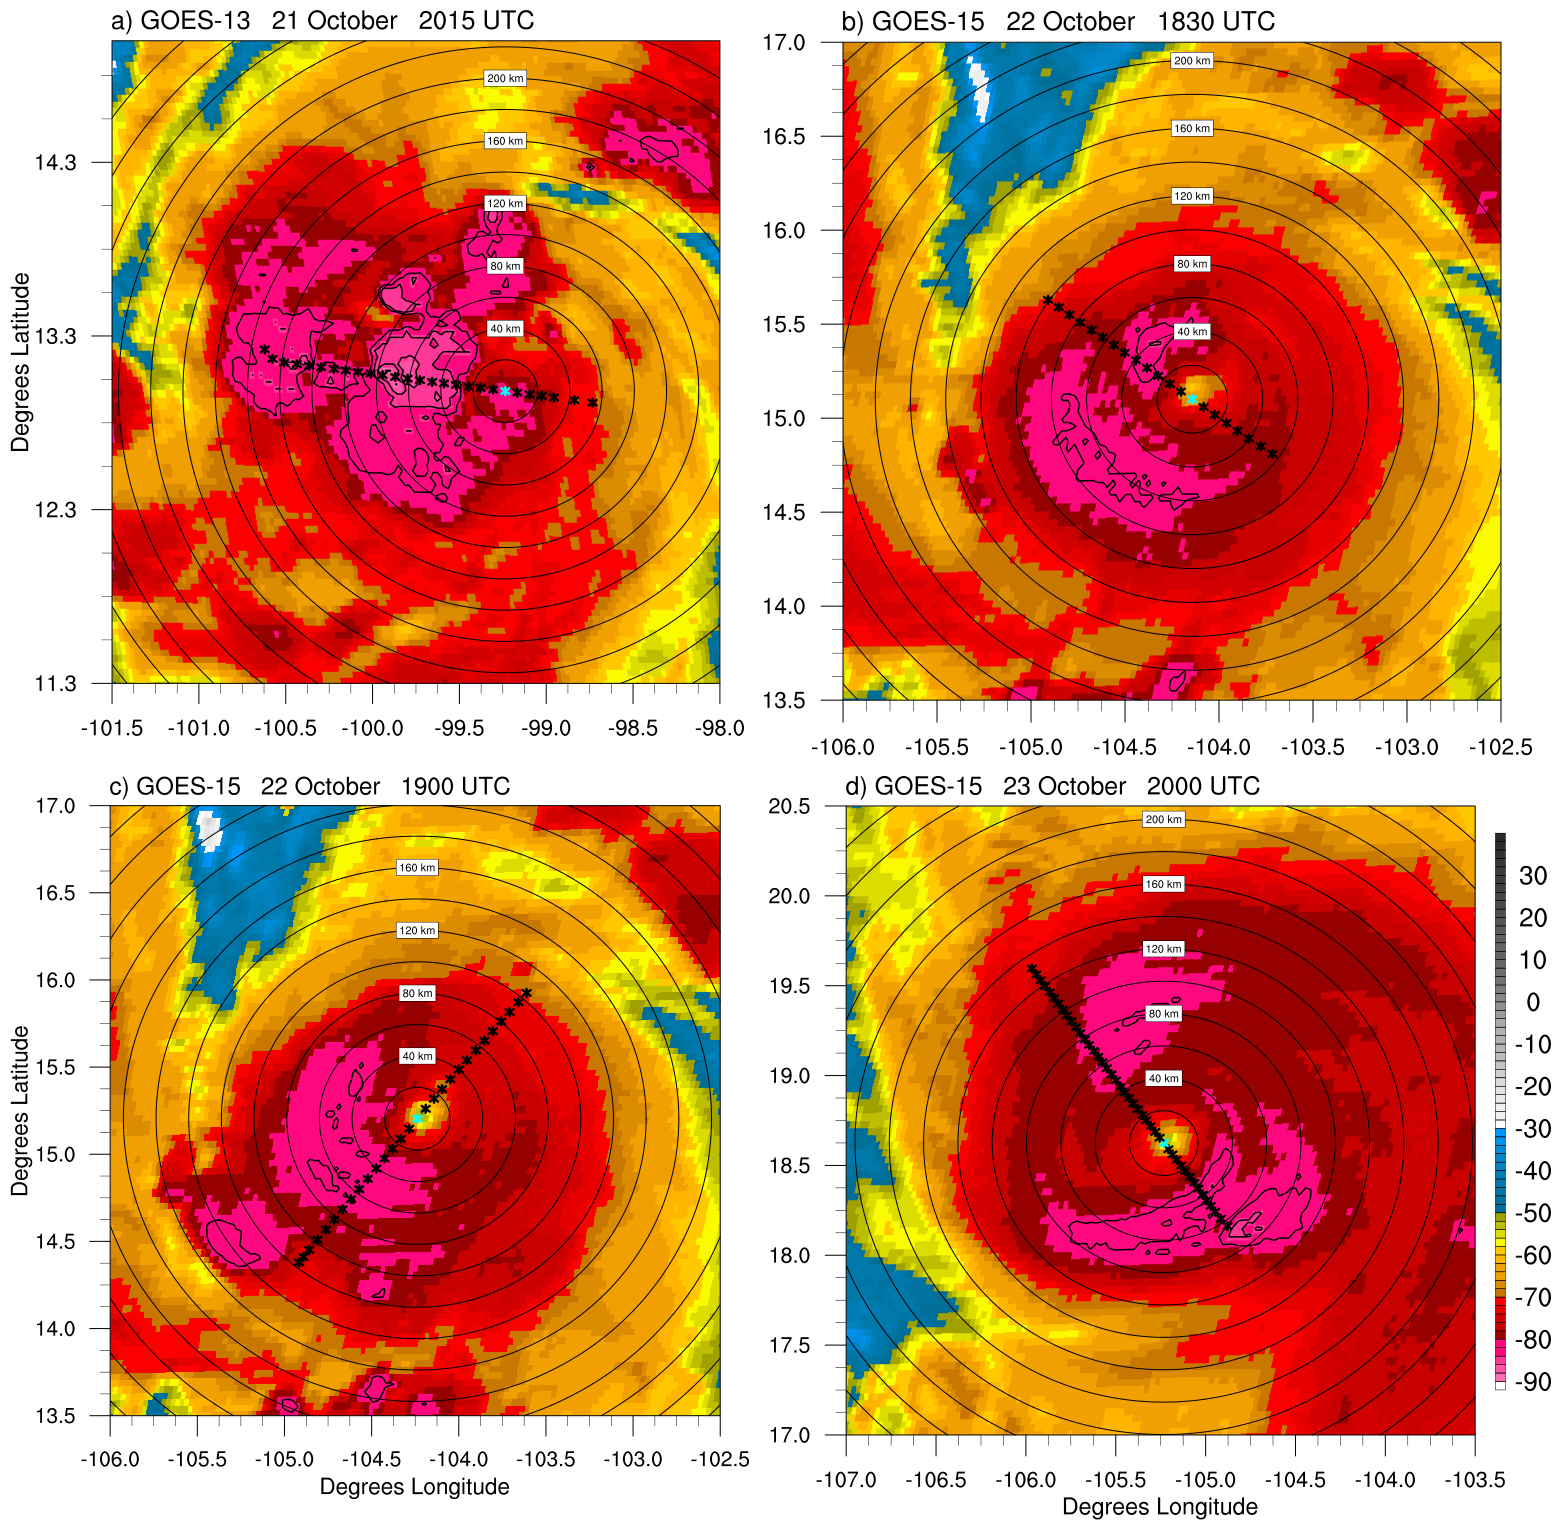
\includegraphics[width=39pc]{figures/fig01_patricia_ir.png}}
\caption{Infrared brightness temperature (\textdegree{}C) images of Tropical Storm Patricia at (a) 2015 UTC 21 Oct, and Hurricane Patricia at (b) 1830 UTC 22 Oct, (c) 1900 UTC 22 Oct, and (d) 2000 UTC 23 Oct 2015. Stars represent dropsonde deployment locations, with cyan stars marking the center location used for each cross section. Black contours delineate the coldest brightness temperatures, with a contour interval of 2\textdegree{}C starting at -82\textdegree{}C. The mean dropsonde spacing is (a) 7.9, (b) 7.8, (c) 8.0, and (d) 4.4 km for the four flight legs. Range rings are plotted every 20 km.}
\label{fig:patricia_ir}
\end{figure*}

%FIGURE 2%
\begin{figure*}[ht]
\centerline{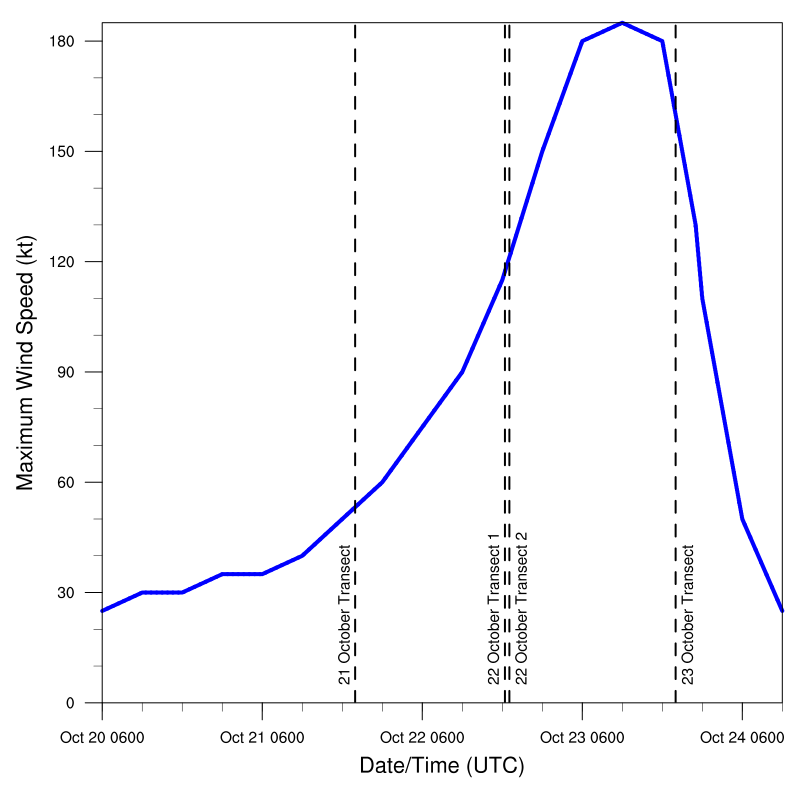
\includegraphics[width=39pc]{figures/fig02_patricia-intensity.png}}
\caption{The maximum wind speed (kt; blue line) throughout Patricia’s lifetime recorded in the National Hurricane Center best track \citep{Kimberlainetal2016}. Vertical lines indicate the times at which the WB-57 passed over the storm center during the four transects shown in Fig. \ref{fig:patricia_ir}.}
\label{fig:vmax}
\end{figure*}

%FIGURE 3%
\begin{figure*}[ht]
\centerline{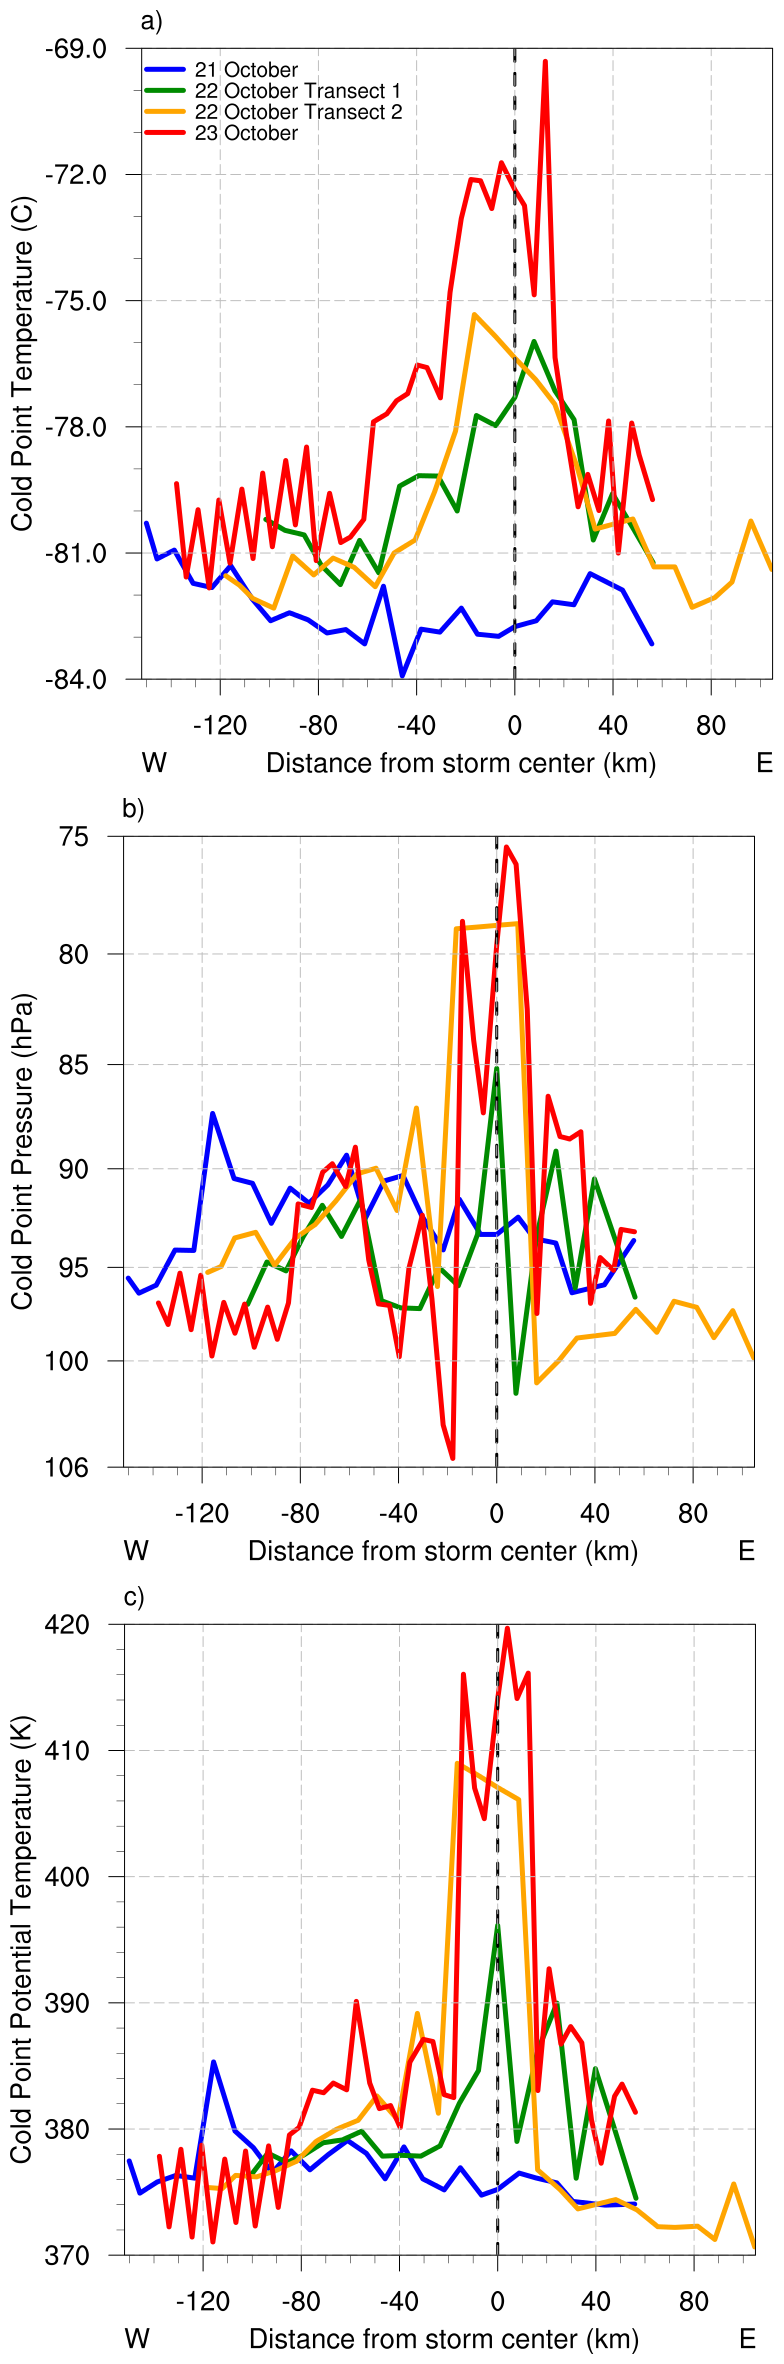
\includegraphics[width=16pc]{figures/fig03_cp_temp+theta+pres.png}}
\caption{(a) Temperature (\textdegree{}C), (b) pressure (hPa), and (c) potential temperature (K) at the cold-point tropopause for flights through the center of Tropical Storm Patricia at 1957 UTC 21 Oct (blue), and Hurricane Patricia at 1823 UTC 22 Oct (green), 1906} UTC 22 Oct (orange), and 2001 UTC 23 Oct (red) 2015. The vertical dashed lines represent the storm center. Compass directions are indicated by letters at each end of the cross section.
\label{fig:trop}
\end{figure*}

%FIGURE 4%
\begin{figure*}[ht]
\centerline{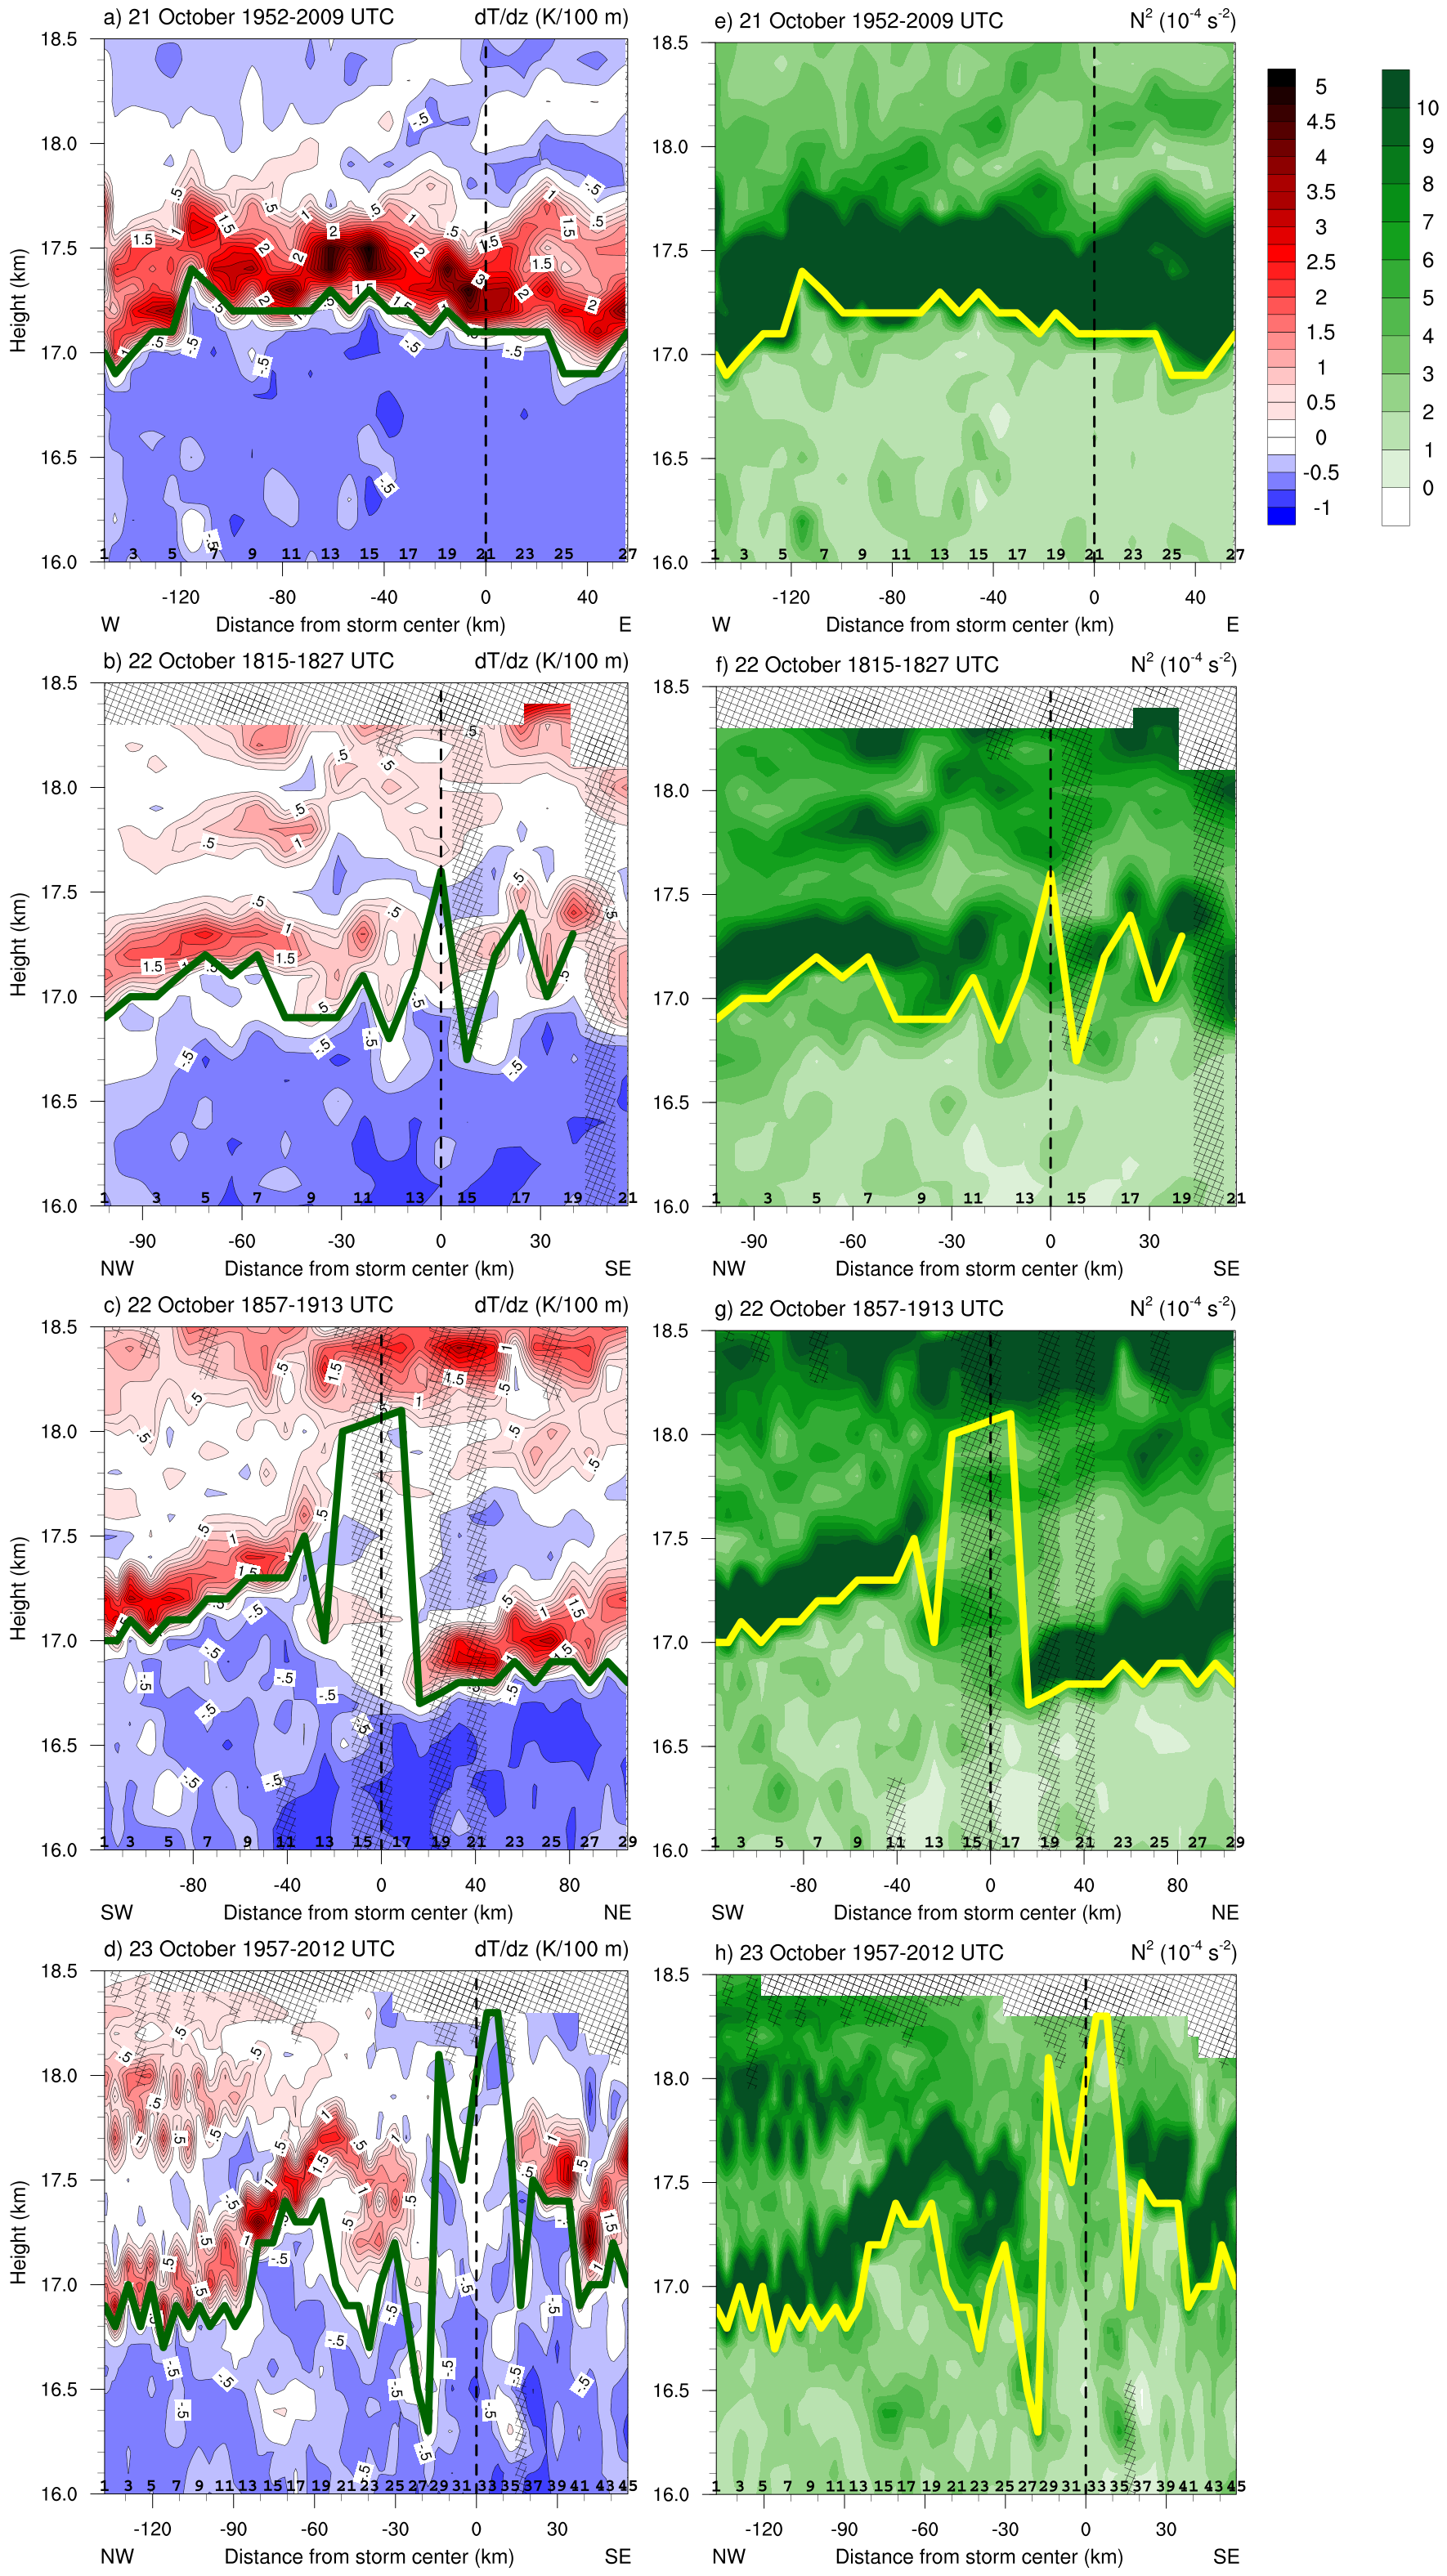
\includegraphics[width=24pc]{figures/fig04_dtdz+stab.png}}
\caption{(left) Vertical cross sections of $\Delta T/\Delta z$ [K (100 m)\textsuperscript{-1}; filled contours] and the cold-point tropopause height (green lines) along the transects shown in Fig. 1 on (a) 21; (b),(c) 22; and (d) 23 Oct 2015. Numbers along the bottom of each cross section represent the dropsonde deployment locations shown in Fig. 1 (only odd-numbered dropsondes are labeled here), with number 1 corresponding to the westernmost dropsonde. Compass directions are indicated by letters at each end of the cross sections. Dashed vertical lines mark the storm center and hatching indicates regions of missing values, where linear interpolation is performed in the radial direction. (right) Vertical cross sections of Brunt–Väisälä frequency squared (10\textsuperscript{-4} s\textsuperscript{-2}; filled contours) and cold-point tropopause height (yellow lines) on (e) 21; (f),(g) 22; and (h) 23 Oct 2015.}
\label{fig:stab}
\end{figure*}

%FIGURE 5%
\begin{figure*}[ht]
\centerline{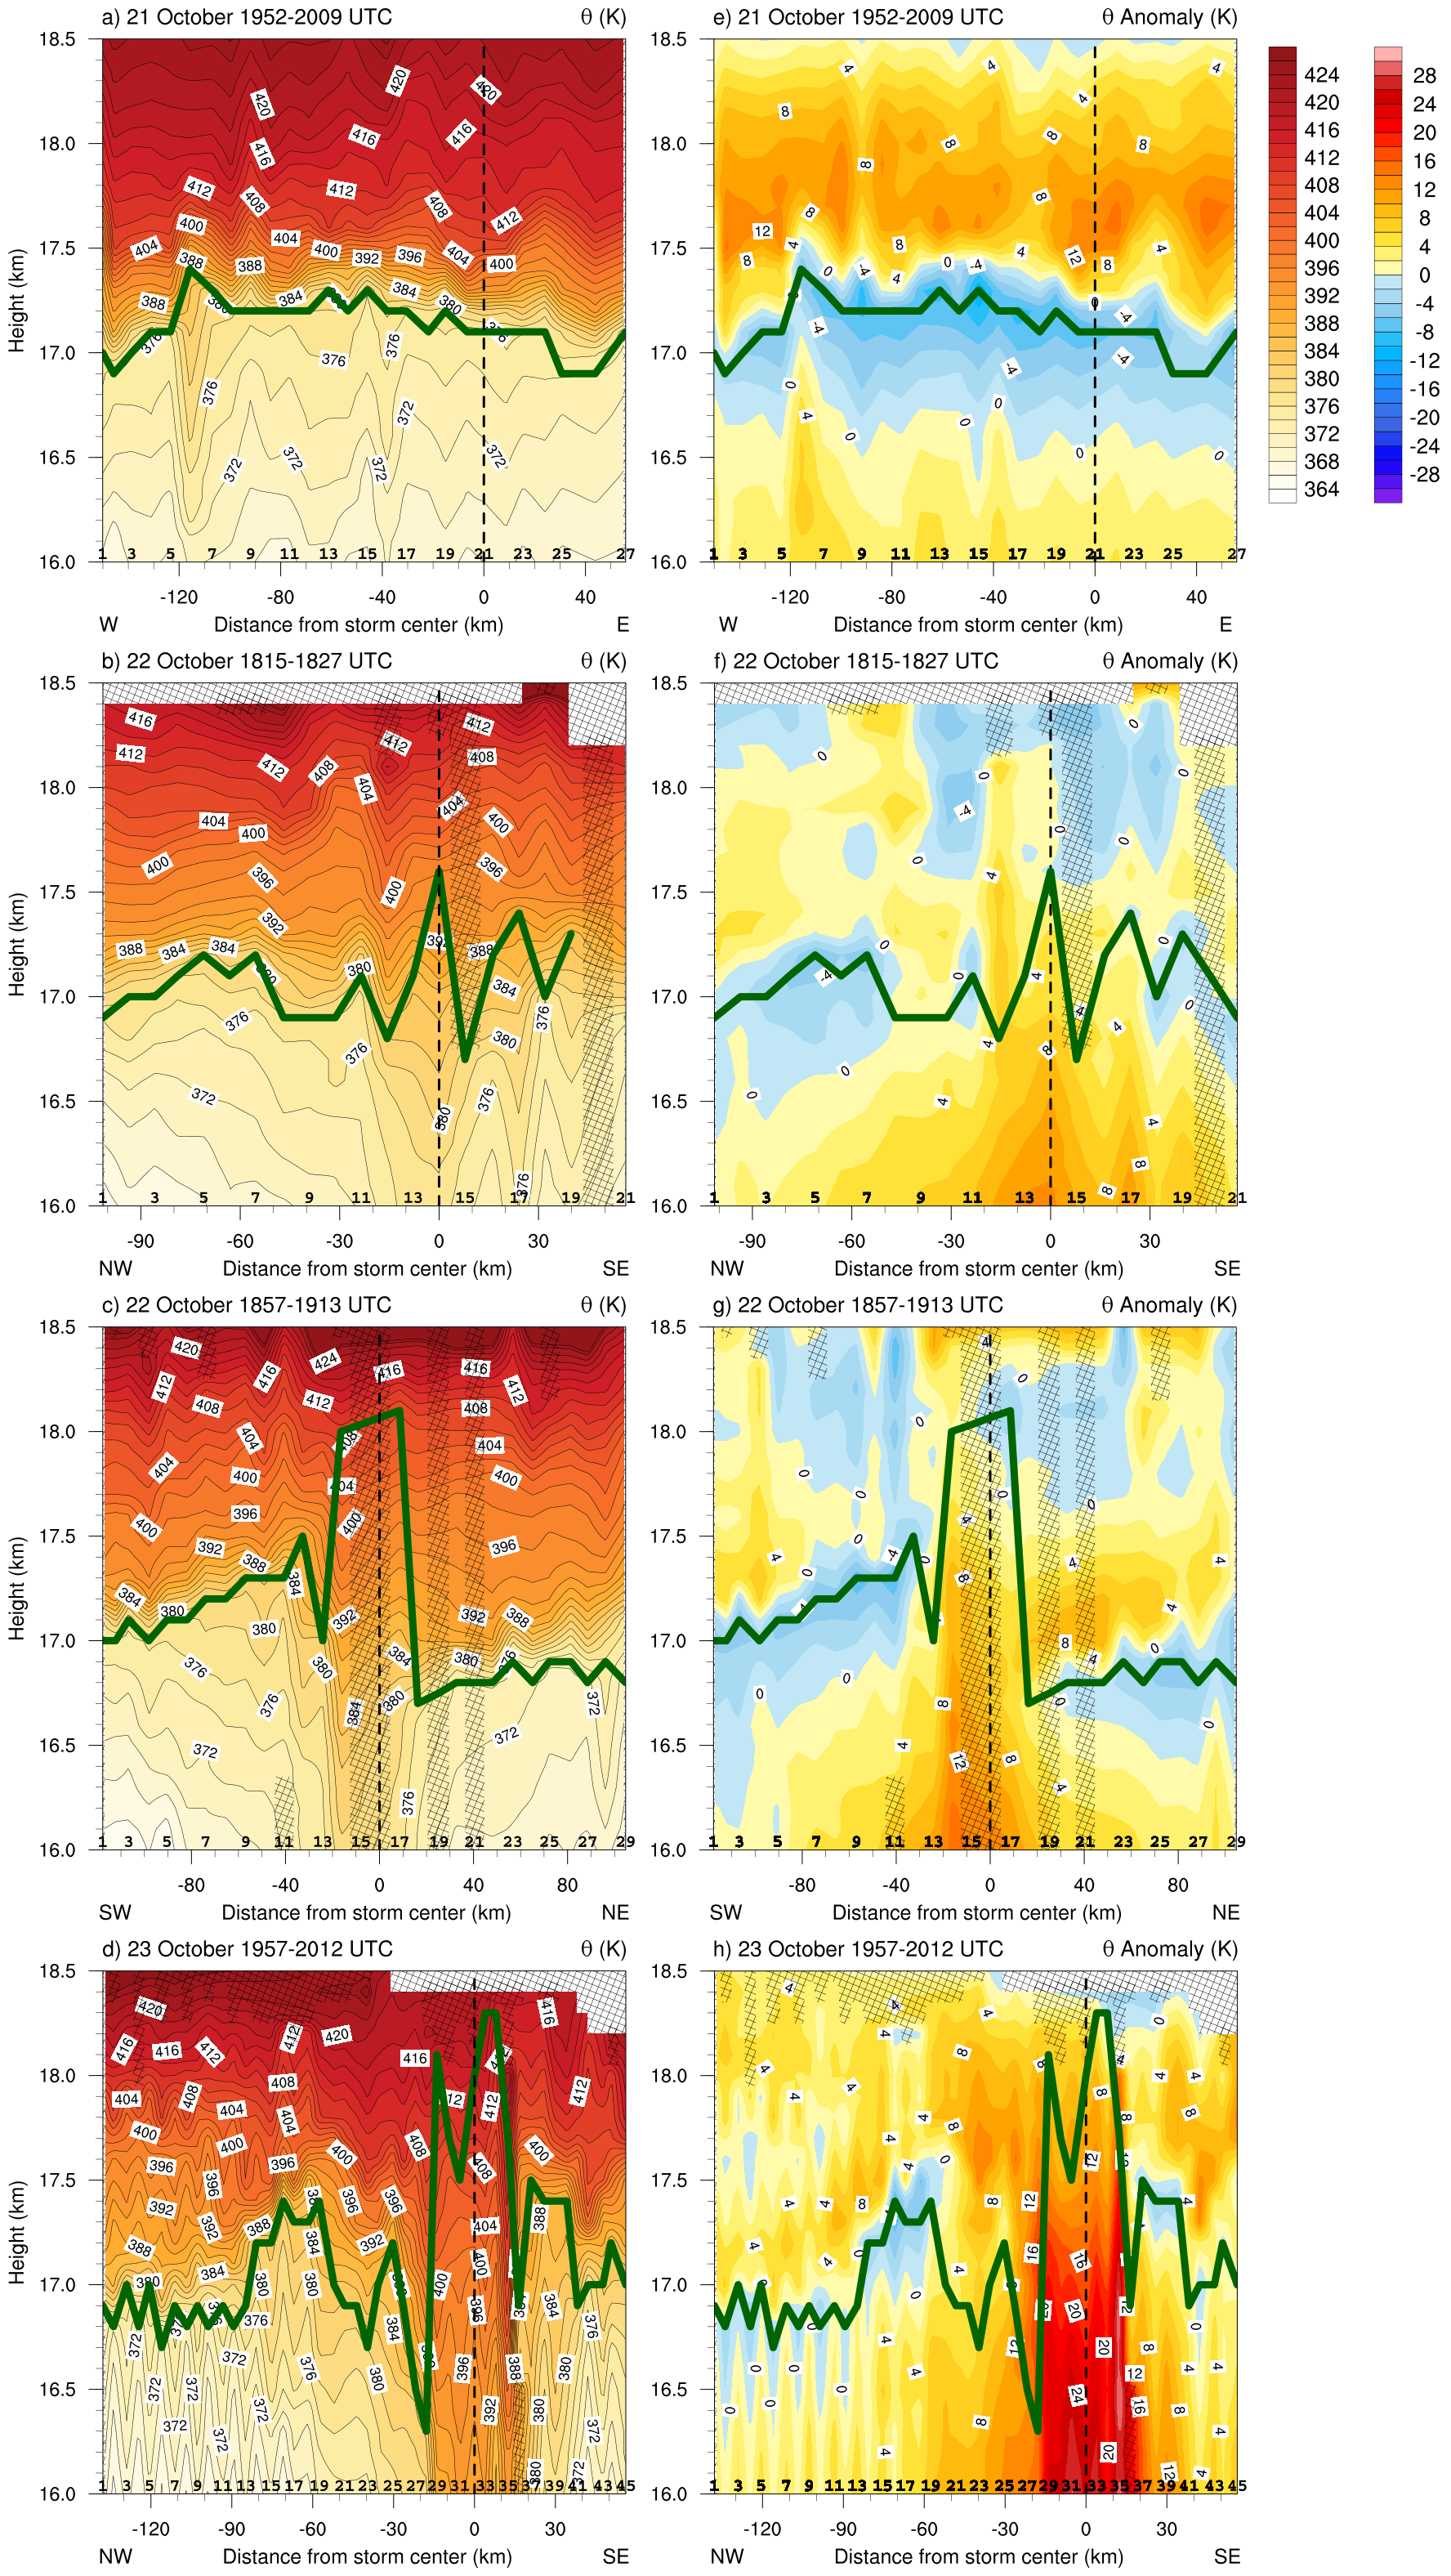
\includegraphics[width=24pc]{figures/fig05_theta+anomalies.png}}
\caption{(left) Vertical cross sections of potential temperature (\textdegree{}C; filled contours) and the cold-point tropopause height (green lines) along the transects shown in Fig. 1 on (a) 21; (b), (c) 22; and (d) 23 Oct 2015. Dropsonde locations, compass directions, and hatching as in Fig. \ref{fig:stab}. (right) Vertical cross sections of the potential temperature anomaly (\textdegree{}C) on (e) 21; (f),(g) 22; and (h) 23 Oct 2015.}
\label{fig:anomalies}
\end{figure*}

%FIGURE 6%
\begin{figure*}[ht]
\centerline{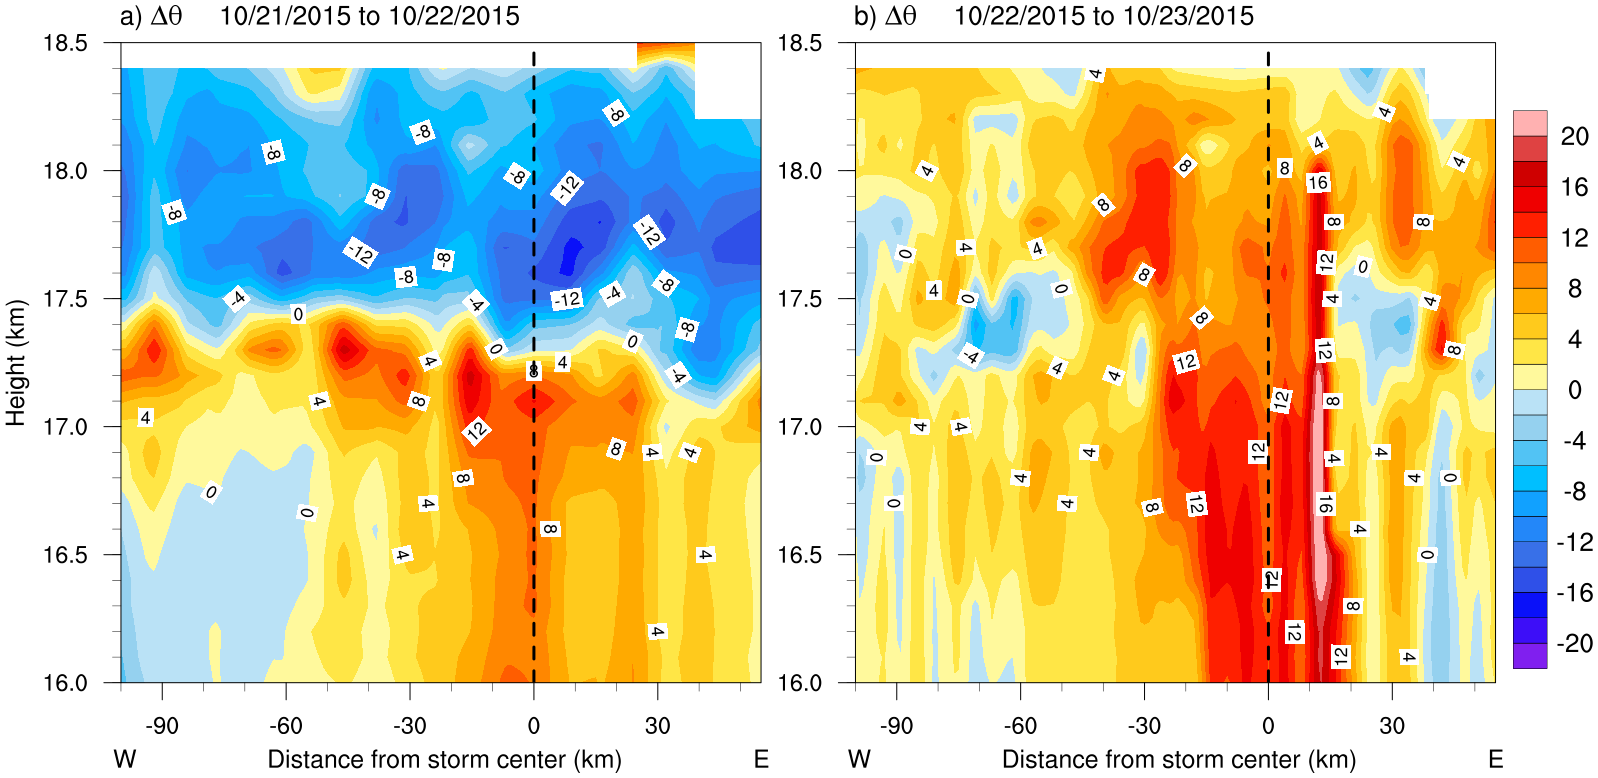
\includegraphics[width=39pc]{figures/fig06_deltatheta.png}}
\caption{Vertical cross sections of the potential temperature change (K day\textsuperscript{-1}) from (a) 21 to 22 Oct and (b) 22 to 23 Oct. These panels extend from the 100-km radius in Patricia’s western semicircle to 55 km in the eastern semicircle. The times separating the transects ($\Delta t$) were 22.45 h (21–22 Oct) and 25.63 h (22–23 Oct). To ease comparison between the two time periods, the potential temperature changes are scaled to 24 h by multiplying by ($24/\Delta t$).}
\label{fig:dtheta}
\end{figure*}

%FIGURE 7%
\begin{figure*}[ht]
\centerline{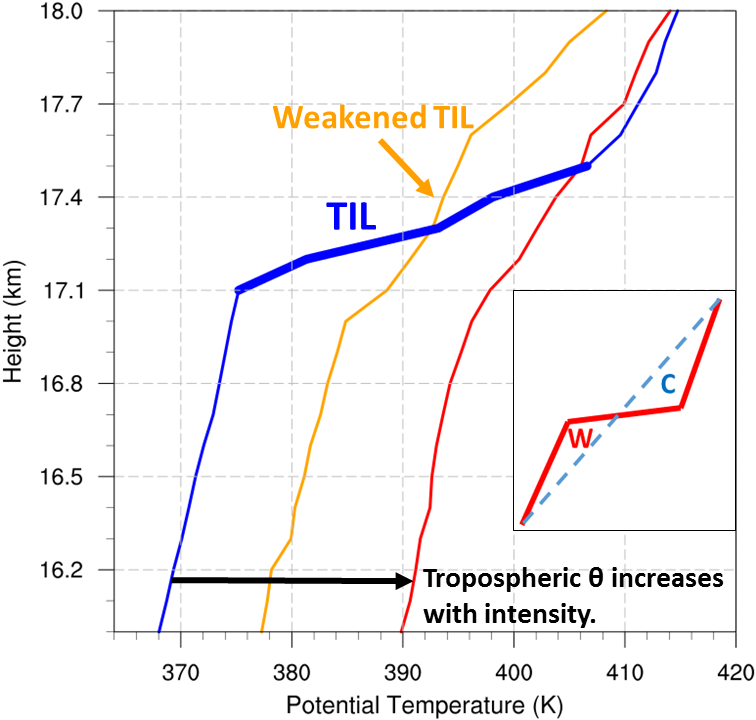
\includegraphics[width=33pc]{figures/fig07_schematic.png}}
\caption{Vertical profiles of potential temperature (K) between 16- and 18-km height for the soundings at Patricia’s storm center on 21 Oct (blue), 22 Oct (orange), and 23 Oct 2015 (red). The bolded segment of the blue line denotes the TIL on 21 Oct. (inset) A simplified schematic of mixing across a strongly stable layer, with the solid red line indicating the initial potential temperature profile and the dashed blue line representing the profile after a period of mixing; ‘‘W’’ and ‘‘C’’ represent regions of warming and cooling, respectively, after mixing.}
\label{fig:schematic}
\end{figure*}

%FIGURE 8%
\begin{figure*}[ht]
\centerline{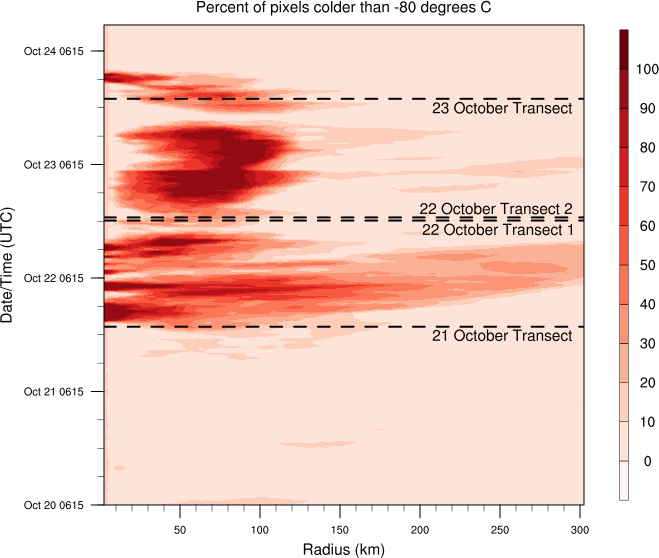
\includegraphics[width=39pc]{figures/fig08_hovmoller_tbpercent.png}}
\caption{Radius–time plot of the percent of infrared brightness temperature pixels colder than -80\textdegree{}C. The plot is constructed by counting the number of pixels colder than -80\textdegree{}C in a 5-km-wide radial bin, dividing by the total number of pixels in that bin, and multiplying by 100. This is performed every 5 km, extending from the storm center out to 300-km radius, for each GOES-13 image collected during Patricia’s lifetime (images are available every 30 min). Dashed black lines mark the times at which the WB-57 aircraft crossed over the storm center.}
\label{fig:hovmoller}
\end{figure*}

%FIGURE 9%
\begin{figure*}[ht]
\centerline{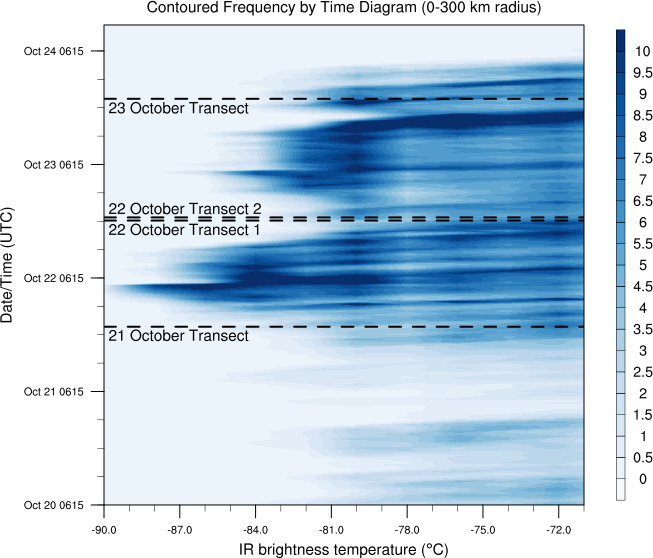
\includegraphics[width=39pc]{figures/fig09_CFTD.png}}
\caption{Contoured frequency by time diagram of infrared (IR) brightness temperature (\textdegree{}C) for all IR pixels within 300 km of the storm center observed by GOES-13 throughout Patricia’s lifetime. The plot is constructed by sampling the full distribution of IR brightness temperature within 300 km of the storm center and determining the percentage of pixels that fall into each IR brightness temperature bin (using 2-K-wide bins). Dashed black lines mark the times at which the WB-57 aircraft crossed over the
storm center.}
\label{fig:CFTD}
\end{figure*}

%FIGURE 10%
\begin{figure*}[ht]
\centerline{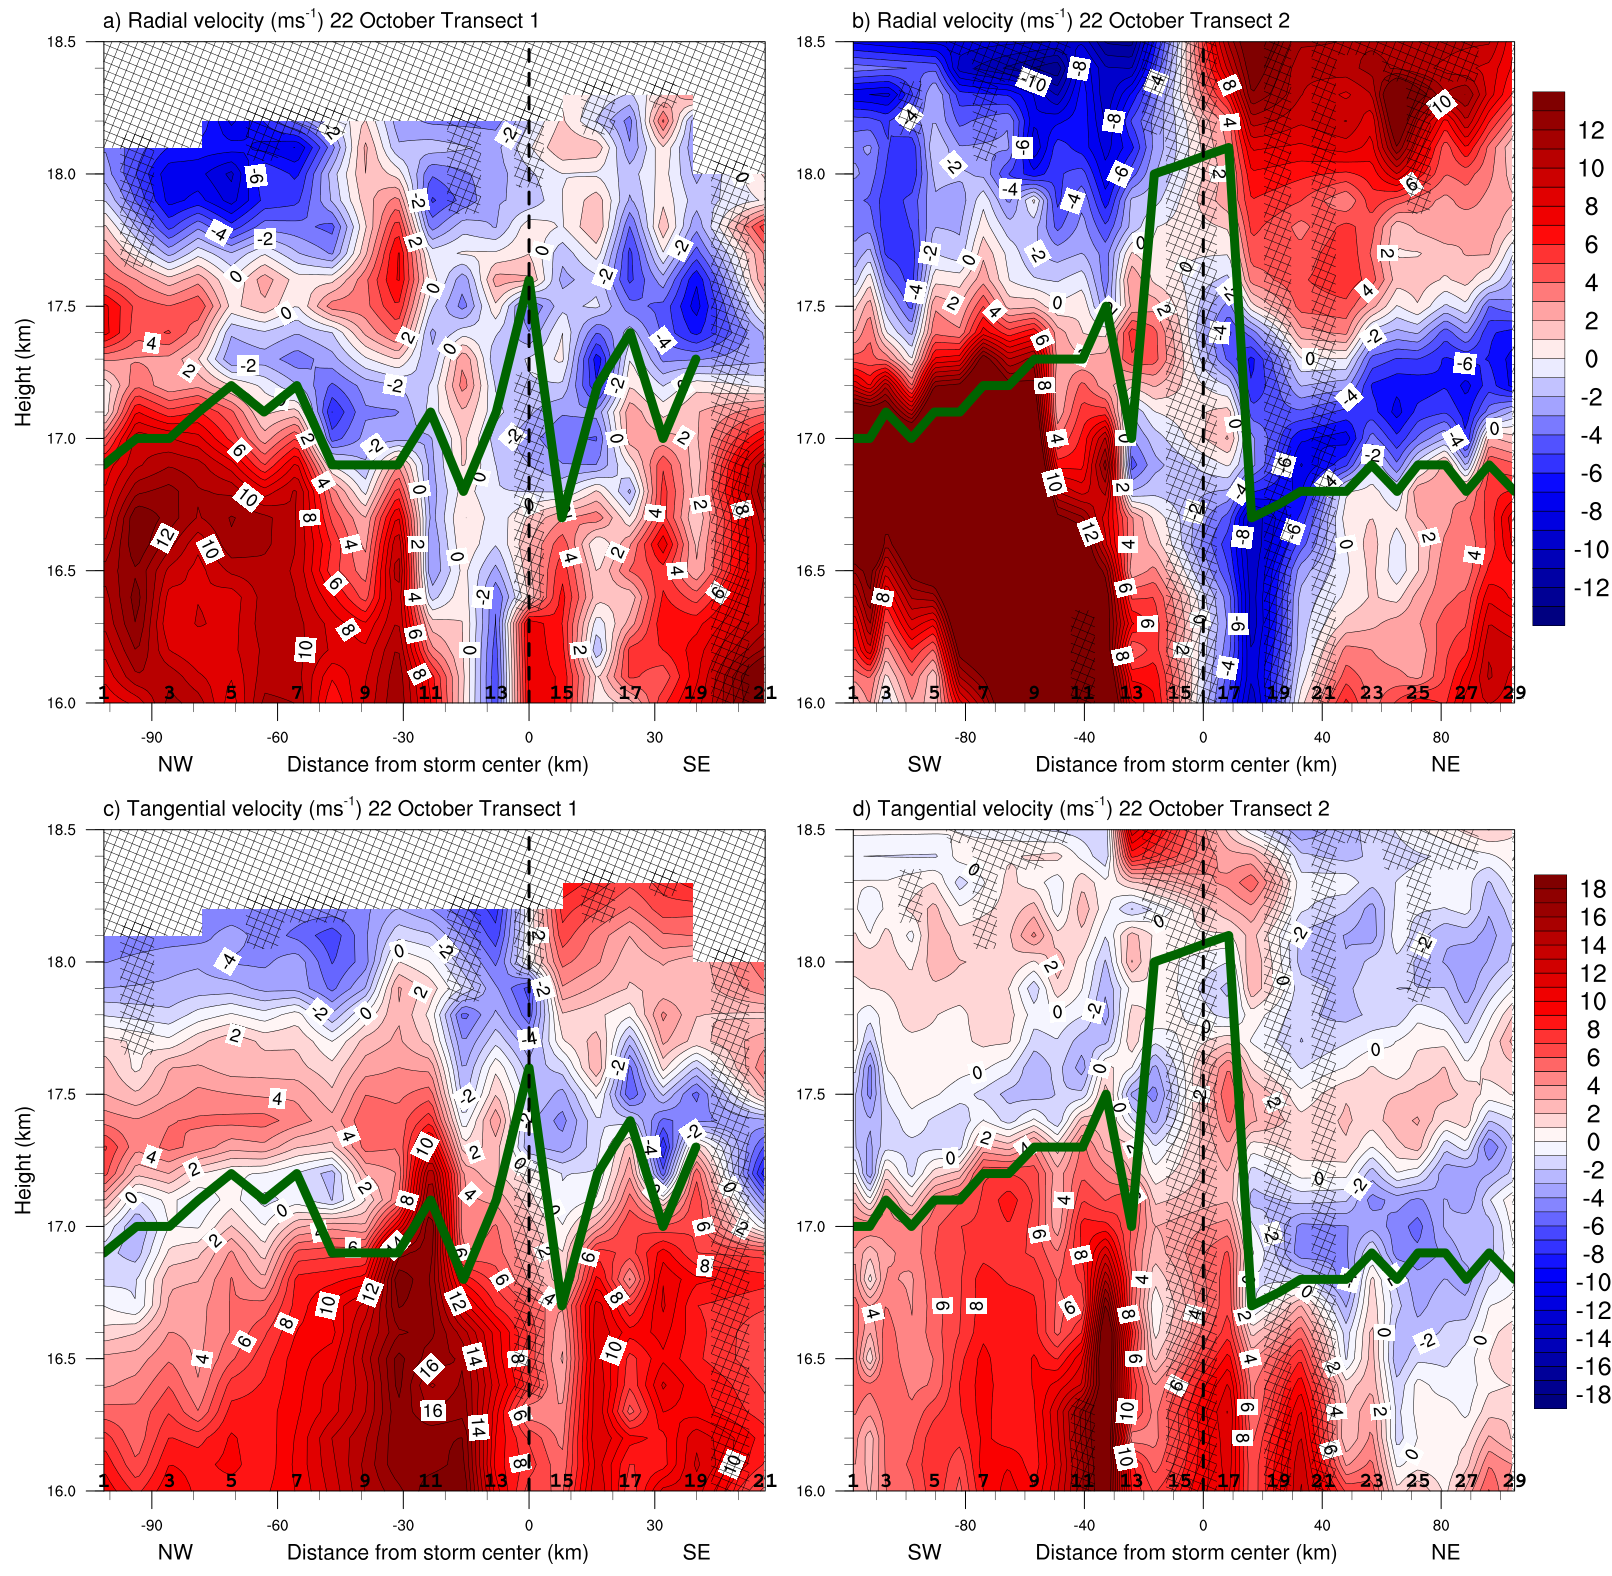
\includegraphics[width=39pc]{figures/fig10_velocities.png}}
\caption{Vertical cross sections of (a),(b) storm-relative radial and (c),(d) tangential velocity (m s\textsuperscript{-1}) and the cold-point tropopause height (green lines) in Hurricane Patricia for the two center-crossing transects on 22 Oct 2015. Dropsonde locations, compass directions, and vertical hatching as in Fig. \ref{fig:stab}.}
\label{fig:velocities}
\end{figure*}
